\documentclass{article}
\usepackage{tikz}
\usetikzlibrary{arrows.meta}

\begin{document}

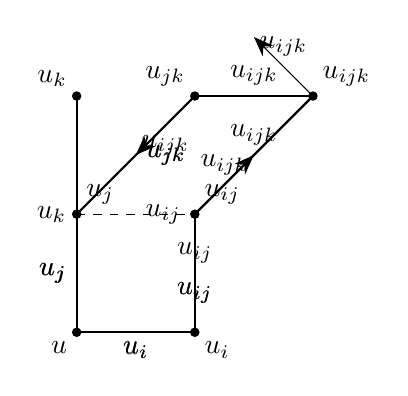
\begin{tikzpicture}[scale=1.5]
    % Define coordinates
    \coordinate (u) at (0,0);
    \coordinate (ui) at (1,0);
    \coordinate (uj) at (0,1);
    \coordinate (uk) at (0,2);
    \coordinate (uij) at (1,1);
    \coordinate (ujk) at (1,2);
    \coordinate (uijk) at (2,2);

    % Draw edges
    \draw[thick] (u) -- (ui) node [midway, below] {$u_i$};
    \draw[thick] (u) -- (uj) node [midway, left] {$u_j$};
    \draw[thick] (u) -- (uk) node [midway, left] {$u_k$};
    \draw[thick] (ui) -- (uij) node [midway, above] {$u_{ij}$};
    \draw[thick] (uj) -- (ujk) node [midway, right] {$u_{jk}$};
    \draw[thick] (uij) -- (uijk) node [midway, above] {$u_{ijk}$};
    \draw[thick] (ujk) -- (uijk) node [midway, above] {$u_{ijk}$};

    % Draw dashed edges
    \draw[dashed] (u) -- (uj) node [midway, left] {$u_j$};
    \draw[dashed] (u) -- (ui) node [midway, below] {$u_i$};
    \draw[dashed] (uj) -- (uij) node [midway, right] {$u_{ij}$};
    \draw[dashed] (ui) -- (uij) node [midway, below] {$u_{ij}$};
    \draw[dashed] (uj) -- (ujk) node [midway, right] {$u_{jk}$};
    \draw[dashed] (ui) -- (uij) node [midway, below] {$u_{ij}$};

    % Draw arrows
    \draw[-{Stealth[scale=1.5]}] (uij) -- ++(0.5,0.5) node [midway, above] {$u_{ijk}$};
    \draw[-{Stealth[scale=1.5]}] (ujk) -- ++(-0.5,-0.5) node [midway, below] {$u_{ijk}$};
    \draw[-{Stealth[scale=1.5]}] (uijk) -- ++(-0.5,0.5) node [midway, above] {$u_{ijk}$};

    % Mark points
    \filldraw[black] (u) circle (1pt) node [below left] {$u$};
    \filldraw[black] (ui) circle (1pt) node [below right] {$u_i$};
    \filldraw[black] (uj) circle (1pt) node [above right] {$u_j$};
    \filldraw[black] (uk) circle (1pt) node [above left] {$u_k$};
    \filldraw[black] (uij) circle (1pt) node [above right] {$u_{ij}$};
    \filldraw[black] (ujk) circle (1pt) node [above left] {$u_{jk}$};
    \filldraw[black] (uijk) circle (1pt) node [above right] {$u_{ijk}$};
\end{tikzpicture}

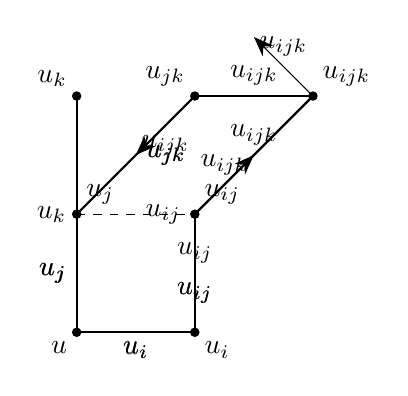
\begin{tikzpicture}[scale=1.5]
    % Define coordinates
    \coordinate (u) at (0,0);
    \coordinate (ui) at (1,0);
    \coordinate (uj) at (0,1);
    \coordinate (uk) at (0,2);
    \coordinate (uij) at (1,1);
    \coordinate (ujk) at (1,2);
    \coordinate (uijk) at (2,2);

    % Draw edges
    \draw[thick] (u) -- (ui) node [midway, below] {$u_i$};
    \draw[thick] (u) -- (uj) node [midway, left] {$u_j$};
    \draw[thick] (u) -- (uk) node [midway, left] {$u_k$};
    \draw[thick] (ui) -- (uij) node [midway, above] {$u_{ij}$};
    \draw[thick] (uj) -- (ujk) node [midway, right] {$u_{jk}$};
    \draw[thick] (uij) -- (uijk) node [midway, above] {$u_{ijk}$};
    \draw[thick] (ujk) -- (uijk) node [midway, above] {$u_{ijk}$};

    % Draw dashed edges
    \draw[dashed] (u) -- (uj) node [midway, left] {$u_j$};
    \draw[dashed] (u) -- (ui) node [midway, below] {$u_i$};
    \draw[dashed] (uj) -- (uij) node [midway, right] {$u_{ij}$};
    \draw[dashed] (ui) -- (uij) node [midway, below] {$u_{ij}$};
    \draw[dashed] (uj) -- (ujk) node [midway, right] {$u_{jk}$};
    \draw[dashed] (ui) -- (uij) node [midway, below] {$u_{ij}$};

    % Draw arrows
    \draw[-{Stealth[scale=1.5]}] (uij) -- ++(0.5,0.5) node [midway, above] {$u_{ijk}$};
    \draw[-{Stealth[scale=1.5]}] (ujk) -- ++(-0.5,-0.5) node [midway, below] {$u_{ijk}$};
    \draw[-{Stealth[scale=1.5]}] (uijk) -- ++(-0.5,0.5) node [midway, above] {$u_{ijk}$};

    % Mark points
    \filldraw[black] (u) circle (1pt) node [below left] {$u$};
    \filldraw[black] (ui) circle (1pt) node [below right] {$u_i$};
    \filldraw[black] (uj) circle (1pt) node [above right] {$u_j$};
    \filldraw[black] (uk) circle (1pt) node [above left] {$u_k$};
    \filldraw[black] (uij) circle (1pt) node [above right] {$u_{ij}$};
    \filldraw[black] (ujk) circle (1pt) node [above left] {$u_{jk}$};
    \filldraw[black] (uijk) circle (1pt) node [above right] {$u_{ijk}$};
\end{tikzpicture}

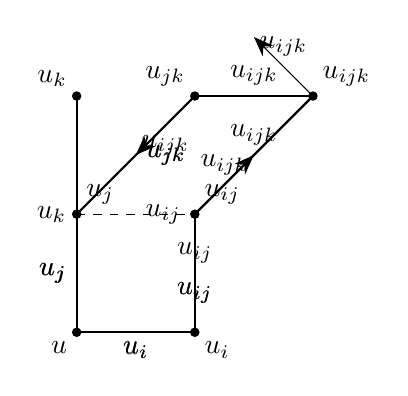
\begin{tikzpicture}[scale=1.5]
    % Define coordinates
    \coordinate (u) at (0,0);
    \coordinate (ui) at (1,0);
    \coordinate (uj) at (0,1);
    \coordinate (uk) at (0,2);
    \coordinate (uij) at (1,1);
    \coordinate (ujk) at (1,2);
    \coordinate (uijk) at (2,2);

    % Draw edges
    \draw[thick] (u) -- (ui) node [midway, below] {$u_i$};
    \draw[thick] (u) -- (uj) node [midway, left] {$u_j$};
    \draw[thick] (u) -- (uk) node [midway, left] {$u_k$};
    \draw[thick] (ui) -- (uij) node [midway, above] {$u_{ij}$};
    \draw[thick] (uj) -- (ujk) node [midway, right] {$u_{jk}$};
    \draw[thick] (uij) -- (uijk) node [midway, above] {$u_{ijk}$};
    \draw[thick] (ujk) -- (uijk) node [midway, above] {$u_{ijk}$};

    % Draw dashed edges
    \draw[dashed] (u) -- (uj) node [midway, left] {$u_j$};
    \draw[dashed] (u) -- (ui) node [midway, below] {$u_i$};
    \draw[dashed] (uj) -- (uij) node [midway, right] {$u_{ij}$};
    \draw[dashed] (ui) -- (uij) node [midway, below] {$u_{ij}$};
    \draw[dashed] (uj) -- (ujk) node [midway, right] {$u_{jk}$};
    \draw[dashed] (ui) -- (uij) node [midway, below] {$u_{ij}$};

    % Draw arrows
    \draw[-{Stealth[scale=1.5]}] (uij) -- ++(0.5,0.5) node [midway, above] {$u_{ijk}$};
    \draw[-{Stealth[scale=1.5]}] (ujk) -- ++(-0.5,-0.5) node [midway, below] {$u_{ijk}$};
    \draw[-{Stealth[scale=1.5]}] (uijk) -- ++(-0.5,0.5) node [midway, above] {$u_{ijk}$};

    % Mark points
    \filldraw[black] (u) circle (1pt) node [below left] {$u$};
    \filldraw[black] (ui) circle (1pt) node [below right] {$u_i$};
    \filldraw[black] (uj) circle (1pt) node [above right] {$u_j$};
    \filldraw[black] (uk) circle (1pt) node [above left] {$u_k$};
    \filldraw[black] (uij) circle (1pt) node [above right] {$u_{ij}$};
    \filldraw[black] (ujk) circle (1pt) node [above left] {$u_{jk}$};
    \filldraw[black] (uijk) circle (1pt) node [above right] {$u_{ijk}$};
\end{tikzpicture}

Multidimensional consistency demands that all three of these routes to calculate \( u_{ijk} \) from initial values \( u, u_i, u_j, u_k \) produce the same value.

\end{document}